
%(BEGIN_QUESTION)
% Copyright 2008, Tony R. Kuphaldt, released under the Creative Commons Attribution License (v 1.0)
% This means you may do almost anything with this work of mine, so long as you give me proper credit

Shown here is a distillation tower, used to separate a liquid mixture of substances into its constituent components.  The process of {\it distillation}, or {\it fractionation} as it is sometimes called, is very common in heavy process industries, most notably petrochemical processing:
 
$$\includegraphics[width=15.5cm]{i03215x01.eps}$$

Distillation of this nature works on the principle of different boiling points.  The distillation of alcohol (to separate a water/alcohol mix in order to obtain a purer alcohol product) is a well-known application of this technology.  In a fractionation tower, the process of boiling and condensation of the mixture's constituent components is repeated endlessly, assuring a high degree of separation between them.

The light vapors extracted from the top of a distillation tower are re-condensed into an ``accumulator'' vessel and re-introduced into the fractionation process as ``reflux.''  The heavy vapors condensing at the bottom of the tower are re-boiled into vapor form again and re-introduced into the fractionation process as ``boil-up.''  It is necessary for reflux and boil-up to be re-introduced into the tower in order to purify the final products as much as possible.  The P\&ID shown here is devoid of any instrumentation for the sake of simplicity.

Looking closer at the reboiler process loop, we see that the flow out of the bottom of the tower splits: part of it goes out as finished ``bottom'' product while the rest goes through the reboiler to re-enter the fractionator as ``boil-up''.  This split is accomplished with a pair of split-range level control valves:

$$\includegraphics[width=15.5cm]{i03215x02.eps}$$

Suppose both the transmitter and the controller are direct-acting (increased level = increased output signal).  Determine the proper calibration ranges for both of these valves.  It may be helpful to express the valve ranges graphically on this scale, showing where along the 4-20 mA controller output signal range each valve will be fully open, fully shut, etc.:

$$\includegraphics[width=15.5cm]{i03215x03.eps}$$

\vskip 20pt \vbox{\hrule \hbox{\strut \vrule{} {\bf Suggestions for Socratic discussion} \vrule} \hrule}

\begin{itemize}
\item{} A good idea in this control system is to install a {\it minimum travel stop} in level valve A, so that it cannot close beyond a certain point.  Explain why this might be important to the overall control of the fractionation tower.
\end{itemize}

\underbar{file i03215}
%(END_QUESTION)





%(BEGIN_ANSWER)

This application requires {\it complementary} split-ranging:

$$\includegraphics[width=15.5cm]{i03215x04.eps}$$
 
%(END_ANSWER)





%(BEGIN_NOTES)

The same split-range valve action may also be used on the reflux loop of the fractionator as well, to control liquid level in the overhead accumulator drum.

\vskip 10pt

A minimum stop on level valve A would be a good idea so that the reboiler is still able to maintain temperature control for the bottom of the tower.  Otherwise, if level valve A were to ever fully close, the reboiler would be unable to push heat into the tower, thus adversely affecting temperature control!

%INDEX% Final Control Elements, valve: split ranging
%INDEX% Process: distillation (generic)

%(END_NOTES)


